\chapter{Future Works}  
  \section{Studies of 2011 PbPb data}

    \subsection{High mass $\gamma-\gamma \rightarrow e^{+} e^{-}$  in PbPb 2011}
      A study of the di-electron production in UPC events is already possible 
  from the recorded 2011 data. 
      This measurement would make use of the electron triggers and combined the 
  current di-muon data with di-electron data from the triggers using the
  ECAL. 
      The electron triggered sample potentially offers a large increase in 
  statistics. 
      By adding the additional channel the statistics would already increase.
      However in addition to this, because of the smaller mass of the electron,
  di-electron production is slightly favor compared to di-muon 
  production.
      STARlight predicts that di-electron cross section is a factor of more than 
  2.5 higher in Xn break-up mode than the di-muons channel when looking 
  at masses above 4 GeV.
      The acceptance for electrons in potential higher as well. 
      The ECAL is position just beyond the tracker, whereas the muon system is 
  outermost sub-detector. 
      This elevates the main reduction of muon acceptance, which is the material
  budget. 
      There is simply a lot a detector in front the muon system.

      In order to perform the study several key additions would need to be made
  relative to the current di-muon analysis. 
      The original reconstruction of the data used in the current di-muon 
  analysis does not contain electron objects. 
      Either the analysis would have to migrated to reconstruction of the data
  done in a newer software version, or reconstruction of the electrons 
  would have to be added to the current analysis chain. 
      There are currently no electron UPC MC samples produced. 
      In order to study the acceptance and efficiency for electrons these samples
  would be need. 
      The ultimate limitation on this study is the 2 GeV threshold in $p_{T}$ in
  the ECAL trigger. 
      This limits the di-electron mass range to where the trigger is efficient. 

      The contribution of higher order diagrams can be explored by the 
  photoproduction of di-lepton pairs is to explore.
      With additional contributions to the physics communities understanding of 
  this process this study will help to determine necessity or 
  non-necessity of including higher order of corrections in simulations 
  such as STARlight.
      Having an additional channel to help constrain the current di-muon measure 
  of the of UPC $\gamma-\gamma$ interaction will also help to constrain 
  the $J/\psi$ measurement by adding a data driven check on the 
  normalization $\gamma-\gamma$ background to the $J/\psi$
      
    \subsection{UPC Hadronic Overlap and PbPb 2011}
      In the model calculations explored in this analysis of UPC quarkonia 
        photoproduction all hadronic interactions are rejected.
      Photoproduction in events where hadronic interactions occur are not 
        included in the cross section calculation.
      However, inclusive $p_{T}$ spectra of $J/\psi$ measured by ALICE in 
        peripheral PbPb collisions show a low momentum peak consistent with 
        coherent photoproduction ~\cite{aliceIclJpsi}.
      \begin{figure}[h]
        \centering
        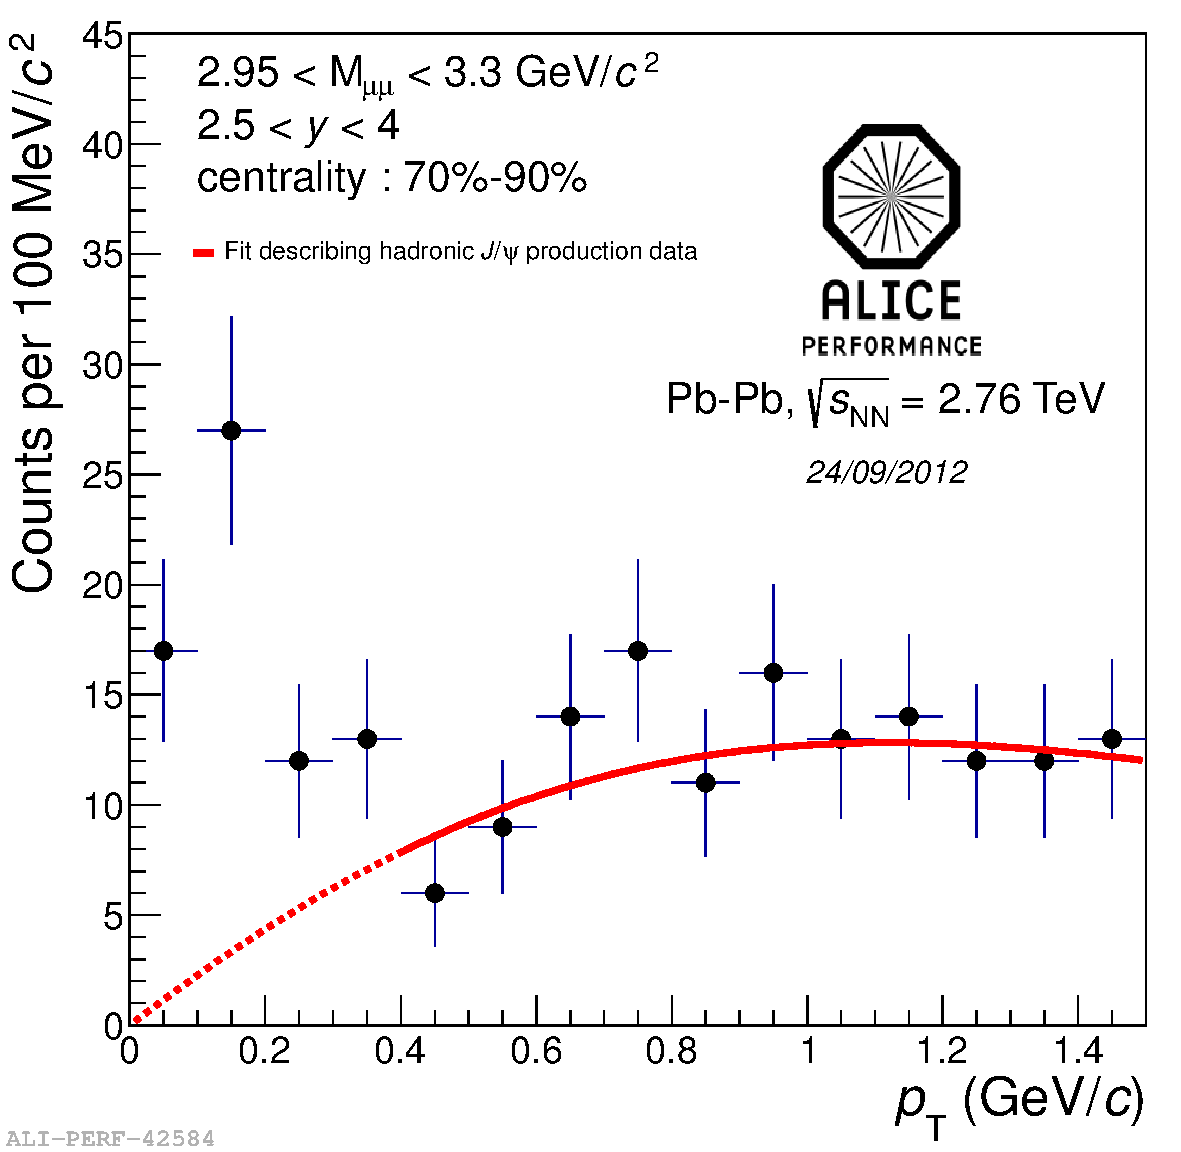
\includegraphics[width=0.5\textwidth]{2012-Sep-24-excess7090.pdf}
        \caption{Coherent excess in inclusive $J/\psi$ $p_{T}$ spectrum.}
        \label{fig:alicePtSpecLowPt}
      \end{figure}
      CMS has the opportunity to explore this overlap between hadronic 
        interactions and photoproduction using PbPb data from 2011 that is 
        already recorded.

      To study the overlap between photoproduction and hadronic proctuction of 
        quarkonia event the inelastic sample and the UPC sample could both be
        used. 
      The looseness of the veto designed to reject hadronic interactions,
        which uses the BSC detector, leaves a significant overlap with 
        peripheral hadronic collisions. 
      The inclusive quarkonia sample from typical hadronic collisions can also 
        be utilized. 
      Coherent quarkonia photoproduction has a distinctive low $p_{T}$ structure
        that can be used to identify photoproduced candidates in a sample that 
        contains photoproduction combined with hadronic interactions.
      This measurement would open up the door to exploring the boundary between
        photoproduction and hadronic production.
      By looking at the mixing of the two, both process, hadronic production and 
        photoproduction, will be better understood.

      In order to compliment each others strengths, the inclusive hadronic sample 
        and the UPC sample of dimuon candidates would be utilized in this study.
      The two samples muon and centrality biases are orthogonal allowing each to 
        serve as a check on the other. 
      The inclusive hadronic sample is triggered by a higher $p_{T}$ threshold 
        double trigger, whereas the UPC sample is uses a lower $p_{T}$ single 
        muon trigger.
      The UPC sample is strongly biased toward peripheral events, which would 
        lead to inefficiencies as events become more central, whereas, the 
        inclusive sample is slightly biases in the most peripheral events due to
        an inefficiency an event selection efficiency in the most peripheral 
        centrality bin.
      If these offsetting biases can be exploited, clarity about the transition 
        between and mixing of photoproduction and hadronic production of 
        quarkonia can be produced. 
      A measurement of the kind proposed here will both produce a better 
        understanding of the low $p_{T}$ portion of the inclusive spectrum as 
        well as the hadronic overlap with UPC measurements.

    \subsection{UPC with muons in HF}
      As higher rapidities are explored both lower and higher momentum partons
        of the nucleus are probed. 
      Because these two contributions to the UPC photoproduction cross section 
        can be separated using neutron tagging in incoherent events, exploring
        higher dimuon rapidities becomes attractive.
      HF extends to 5 in $\eta$, 2.6 units beyond the edge of the tracker.
      By combining hits in HF with tracks in the tracker the higher dimuon 
        rapidities could be explored. 
      When combined with neutron tagging of incoherently produced quarkonia,
        the current study can be extended to probe lower-x nuclear partons 
        by identifying muons in HF. 

  \section{Studies of 2013 pPb data and 2015 PbPb data}
    Specific UPC triggers were also developed for the pPb run in 2013. 
    For this period of running a much higher total trigger rate was read out 
      relative to 2011.
    The total rate allocated for UPC triggers at the L1 in 2013 was 5kHz and 
      50 Hz at the HLT.
    This factor of 5 increase in the bandwidth, especial in L1 rate, allowed for
      a different triggering strategy than in 2011. 

    The basic strategy in 2013 was the same as in 2012, use the loosest 
      available ECAL and muon L1 triggers to push to capture the lowest $p_{T}$
      electrons and muons possible paired with a veto on hadronic interactions,
      but was impemented differently.
    Because of the L1 bandwidth restrictions in 2011, both the ZDC and the BCS 
      were used on the L1 to reduce rates.
    In 2013 only the muon and ECAL triggers were used on the L1 allowing for 
      rejection of hadronic interactions through cuts on track multiplicity. 
    In addition, a more sophisticated trigger using full dimuon reconstructed 
      was developed to increase purity.
    The main advantage in this shift in strategy was a higher purity due to 
      the increased sophistication of the reconstruction on the HLT.
    In addition, an increase in cross section of the underlying physics process
      was achieved by relaxing the neutron emission requirement.

    The PbPb run in 2015 will be at higher beam energies and luminosities.
    The $sqrt{s_{NN}}$ will increase from 2.76 TeV in 2011 to 5.1 TeV with
      a project integrated luminosity between $0.3/nb$ and $1/nb$. 
    The factor of 2 to 10 increase in integrated luminosity will increases the 
      number of events directly.
    In addition, both the increase in energy, which increases the photon flux,
      and the ability to utilize the 2013 trigger strategy of sifting the 
      onus of the trigger selection to the HLT will increase the measured 
      yields relative to 2011.
    The higher beam energy, higher integrated luminosity, and added selectivity
      of the HLT will create the opportunity to explore both $J/\psi$ with 
      greater statistical precision and novel objects such as $\Upsilon$, and 
      jets. 

    \subsection{pPb $J/\psi$}
      $J/\psi$ photoproduciton in pPb collisions is dominated $\gamma-p$ 
        interactions.
      The measurement would primarily probe the proton gluon densities.
      In Eq.~\ref{eq:photonFluxFinaltmp} the photon flux depends on the square
      of the number of protons in parent nucleus, $Z^{2}$. 
      However, the cross section of the target only increase as the total 
        number of nucleons to the 2/3rds power, $A^{2/3}$.
      The much higher photon flux from the Pb ion more than compensates for 
        the decreased size of the proton.

      A pPb UPC $J/\psi$ measurement will compliment the measurements done at 
        HERA, and measurements done by ALICE.
      CMS will contribute by adding additional kinematic coverage and cover a 
        unique range of proton-photon center of mass energies, $W_{p\gamma}$. 
      The difference in beam energies and species at LHC versus HERA result in
        access to different $W_{p\gamma}$. 
      ALICE and CMS have different acceptance in $J/\psi$ rapidity, which also 
        translates to coverage of different $W_{p\gamma}$.
      In addition, an excess in the UPC cross section compared to HERA 
        measurements would indicate a non-exclusive contribution to the pPb UPC 
        $J/\psi$ cross section. 
      This measurement will both help enhance the current understanding of 
        the $p\gamma$ $J/\psi$ photoproduction cross section as a function of 
        $W_{p\gamma}$, and validate the UPCs measurements as an extension of 
        the work done at HERA.

    \subsection{UPC $J/\psi$ and $\Upsilon$ in 2015}
      A measurement of the UPC $J/\psi$ in 2015 will produce a strong constraint
        on the low-x portion of the nuclear gluon distribution relative to 
        the current analysis form the 2011 data. 
      The $J/\psi$ measurement will probe lower-x than in 2011 due to the 
        increase in beam energy. 
      A measurement in 2015 will also have lower statistical errors due to the 
        increase in integrated luminosity and increased L1 bandwidth.
      UPC $J/\psi$s in 2015 will push farther towards the onset of low-x parton 
        saturation.

      Measurement of the UPC $\Upsilon$ cross section from the 2015 data will 
        be the first from PbPb collisions. 
      As with the $J/\psi$, Additional L1 bandwidth, increased beam energy, and
        and intensity will increase the $\Upsilon$ yield significantly relative
        to 2011. 
      CMS's acceptance for $\Upsilon$ is far higher than for $J/\psi$.
      The acceptance for $\Upsilon$ is near 40\% for all rapidities between 
        -2.4 to 2.4.
      Conversely, $J/\psi$ acceptance is 8\% near 2 in dimuon rapidity only. 
      Below 1.6 in rapidity there is not acceptance for for UPC $J/\psi$.
      Estimates from STARlight predict a factor of 17-60 increase in yield
        depending on the total delivered integrated luminosity. 
      The $\Upsilon$ measurement will be a new measurement that will expand the 
        range of x and $Q^{2}$ probed with a higher energy probe that is better
        suited to the acceptance of CMS.

    \subsection{UPC jets}
      Like $\Upsilon$s, UPC photoproduction of jets is a novel probe.
      The LHC 2015 heavy ion run presents an opportunity do this measurement 
        for the first time. 
      The cross section for photoproduction of jets was estimated in 
      Ref~\cite{upcJets1} and found $b\bar{b}$ and $c\bar{c}$ on the order of 
        1 mb and 1b respectively.
      With the integrated luminosity expected for 2015 as many as $1x10^{6}$
        $b\bar{b}$ events and $1x10^{9}$ $c\bar{c}$ events. 
      Jet photoproduction is not constrained by the mass of the bound onia 
        states like in $J/\psi$ and $\Upsilon$ photoproduction. 
      For this reason, jet photoproduction probes a wider range of x and 
        $Q^{2}$.
      UPC jets therefore will both expand on the $J/\psi$ and $\Upsilon$ 
        measurements in addition to providing an additional validating 
        compliment to the onia measurements.

      The jet measurement will require additional trigger development and 
        analysis design. 
      The jet signal differs significantly from the dimuon signals used in the
        current analysis. 
      The trigger scheme used in the 2013 pPb run selected UPC events by 
        vetoing events with high numbers of track. 
      The track multiplicity of the jets will not pass this requirement. 
      However, new L1 trigger logic is currently being developed to separate 
        the jet from the underlaying event in nuclear collisions. 
      This trigger logic could also be utilized to select jet events that
        produce very little to no underlaying event. 
      In addition to the trigger, jet reconstruction algorithms would needed 
        to be adapted to push to the lower pT jets they are produced by 
        photoproduction. 
      The UPC jet measurement will demand extra preparation compared to the 
        onia measurements, but the development will overlap with many of the 
        goals that are already being pursued by the CMS Heavy Ion group and 
        will allow for wider collaboration. 

